\documentclass[twoside]{book}

% Packages required by doxygen
\usepackage{fixltx2e}
\usepackage{calc}
\usepackage{doxygen}
\usepackage[export]{adjustbox} % also loads graphicx
\usepackage{graphicx}
\usepackage[utf8]{inputenc}
\usepackage{makeidx}
\usepackage{multicol}
\usepackage{multirow}
\PassOptionsToPackage{warn}{textcomp}
\usepackage{textcomp}
\usepackage[nointegrals]{wasysym}
\usepackage[table]{xcolor}

% Font selection
\usepackage[T1]{fontenc}
\usepackage[scaled=.90]{helvet}
\usepackage{courier}
\usepackage{amssymb}
\usepackage{sectsty}
\renewcommand{\familydefault}{\sfdefault}
\allsectionsfont{%
  \fontseries{bc}\selectfont%
  \color{darkgray}%
}
\renewcommand{\DoxyLabelFont}{%
  \fontseries{bc}\selectfont%
  \color{darkgray}%
}
\newcommand{\+}{\discretionary{\mbox{\scriptsize$\hookleftarrow$}}{}{}}

% Page & text layout
\usepackage{geometry}
\geometry{%
  a4paper,%
  top=2.5cm,%
  bottom=2.5cm,%
  left=2.5cm,%
  right=2.5cm%
}
\tolerance=750
\hfuzz=15pt
\hbadness=750
\setlength{\emergencystretch}{15pt}
\setlength{\parindent}{0cm}
\setlength{\parskip}{3ex plus 2ex minus 2ex}
\makeatletter
\renewcommand{\paragraph}{%
  \@startsection{paragraph}{4}{0ex}{-1.0ex}{1.0ex}{%
    \normalfont\normalsize\bfseries\SS@parafont%
  }%
}
\renewcommand{\subparagraph}{%
  \@startsection{subparagraph}{5}{0ex}{-1.0ex}{1.0ex}{%
    \normalfont\normalsize\bfseries\SS@subparafont%
  }%
}
\makeatother

% Headers & footers
\usepackage{fancyhdr}
\pagestyle{fancyplain}
\fancyhead[LE]{\fancyplain{}{\bfseries\thepage}}
\fancyhead[CE]{\fancyplain{}{}}
\fancyhead[RE]{\fancyplain{}{\bfseries\leftmark}}
\fancyhead[LO]{\fancyplain{}{\bfseries\rightmark}}
\fancyhead[CO]{\fancyplain{}{}}
\fancyhead[RO]{\fancyplain{}{\bfseries\thepage}}
\fancyfoot[LE]{\fancyplain{}{}}
\fancyfoot[CE]{\fancyplain{}{}}
\fancyfoot[RE]{\fancyplain{}{\bfseries\scriptsize Generated by Doxygen }}
\fancyfoot[LO]{\fancyplain{}{\bfseries\scriptsize Generated by Doxygen }}
\fancyfoot[CO]{\fancyplain{}{}}
\fancyfoot[RO]{\fancyplain{}{}}
\renewcommand{\footrulewidth}{0.4pt}
\renewcommand{\chaptermark}[1]{%
  \markboth{#1}{}%
}
\renewcommand{\sectionmark}[1]{%
  \markright{\thesection\ #1}%
}

% Indices & bibliography
\usepackage{natbib}
\usepackage[titles]{tocloft}
\setcounter{tocdepth}{3}
\setcounter{secnumdepth}{5}
\makeindex

% Hyperlinks (required, but should be loaded last)
\usepackage{ifpdf}
\ifpdf
  \usepackage[pdftex,pagebackref=true]{hyperref}
\else
  \usepackage[ps2pdf,pagebackref=true]{hyperref}
\fi
\hypersetup{%
  colorlinks=true,%
  linkcolor=blue,%
  citecolor=blue,%
  unicode%
}

% Custom commands
\newcommand{\clearemptydoublepage}{%
  \newpage{\pagestyle{empty}\cleardoublepage}%
}

\usepackage{caption}
\captionsetup{labelsep=space,justification=centering,font={bf},singlelinecheck=off,skip=4pt,position=top}

%===== C O N T E N T S =====

\begin{document}

% Titlepage & ToC
\hypersetup{pageanchor=false,
             bookmarksnumbered=true,
             pdfencoding=unicode
            }
\pagenumbering{roman}
\begin{titlepage}
\vspace*{7cm}
\begin{center}%
{\Large My Project }\\
\vspace*{1cm}
{\large Generated by Doxygen 1.8.11}\\
\end{center}
\end{titlepage}
\clearemptydoublepage
\tableofcontents
\clearemptydoublepage
\pagenumbering{arabic}
\hypersetup{pageanchor=true}

%--- Begin generated contents ---
\chapter{Hierarchical Index}
\section{Class Hierarchy}
This inheritance list is sorted roughly, but not completely, alphabetically\+:\begin{DoxyCompactList}
\item Q\+Main\+Window\begin{DoxyCompactList}
\item \contentsline{section}{Main\+Window}{\pageref{class_main_window}}{}
\end{DoxyCompactList}
\item Q\+Widget\begin{DoxyCompactList}
\item \contentsline{section}{Spinor}{\pageref{class_spinor}}{}
\end{DoxyCompactList}
\end{DoxyCompactList}

\chapter{Class Index}
\section{Class List}
Here are the classes, structs, unions and interfaces with brief descriptions\+:\begin{DoxyCompactList}
\item\contentsline{section}{\hyperlink{class_main_window}{Main\+Window} }{\pageref{class_main_window}}{}
\item\contentsline{section}{\hyperlink{class_spinor}{Spinor} }{\pageref{class_spinor}}{}
\end{DoxyCompactList}

\chapter{Class Documentation}
\hypertarget{class_main_window}{}\section{Main\+Window Class Reference}
\label{class_main_window}\index{Main\+Window@{Main\+Window}}
Inheritance diagram for Main\+Window\+:\begin{figure}[H]
\begin{center}
\leavevmode
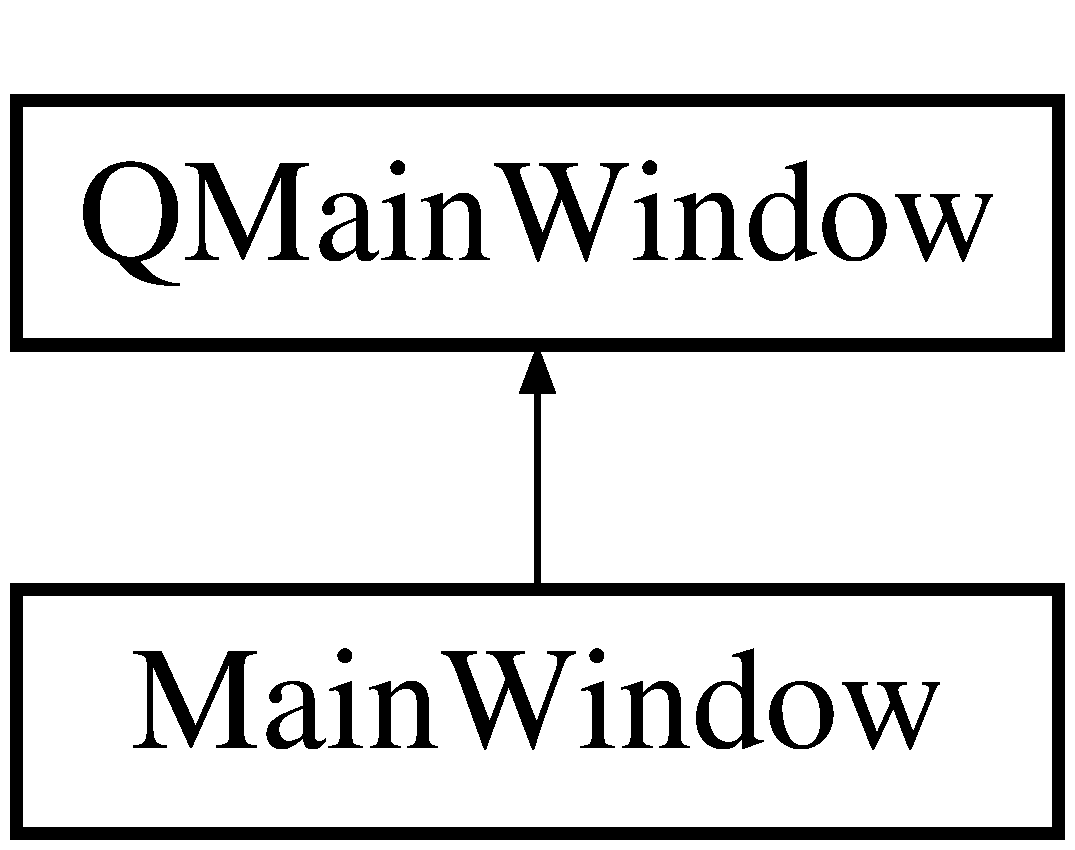
\includegraphics[height=2.000000cm]{class_main_window}
\end{center}
\end{figure}
\subsection*{Public Slots}
\begin{DoxyCompactItemize}
\item 
void {\bfseries easy\+\_\+game} ()\hypertarget{class_main_window_a07a6590ba13449ba65f7c4be6a3908ef}{}\label{class_main_window_a07a6590ba13449ba65f7c4be6a3908ef}

\item 
void {\bfseries normal\+\_\+game} ()\hypertarget{class_main_window_ad99f37fbf0ed64c836a5e63db0edfb7b}{}\label{class_main_window_ad99f37fbf0ed64c836a5e63db0edfb7b}

\item 
void {\bfseries hard\+\_\+game} ()\hypertarget{class_main_window_ae33848e768caf3ebbef0c1461062741f}{}\label{class_main_window_ae33848e768caf3ebbef0c1461062741f}

\item 
void {\bfseries exit} ()\hypertarget{class_main_window_a627d7b538a0d60645e6c339bd787eeee}{}\label{class_main_window_a627d7b538a0d60645e6c339bd787eeee}

\end{DoxyCompactItemize}
\subsection*{Public Member Functions}
\begin{DoxyCompactItemize}
\item 
{\bfseries Main\+Window} (Q\+Widget $\ast$parent=0)\hypertarget{class_main_window_a8b244be8b7b7db1b08de2a2acb9409db}{}\label{class_main_window_a8b244be8b7b7db1b08de2a2acb9409db}

\end{DoxyCompactItemize}


The documentation for this class was generated from the following files\+:\begin{DoxyCompactItemize}
\item 
mainwindow.\+h\item 
mainwindow.\+cpp\end{DoxyCompactItemize}

\hypertarget{class_spinor}{}\section{Spinor Class Reference}
\label{class_spinor}\index{Spinor@{Spinor}}
Inheritance diagram for Spinor\+:\begin{figure}[H]
\begin{center}
\leavevmode
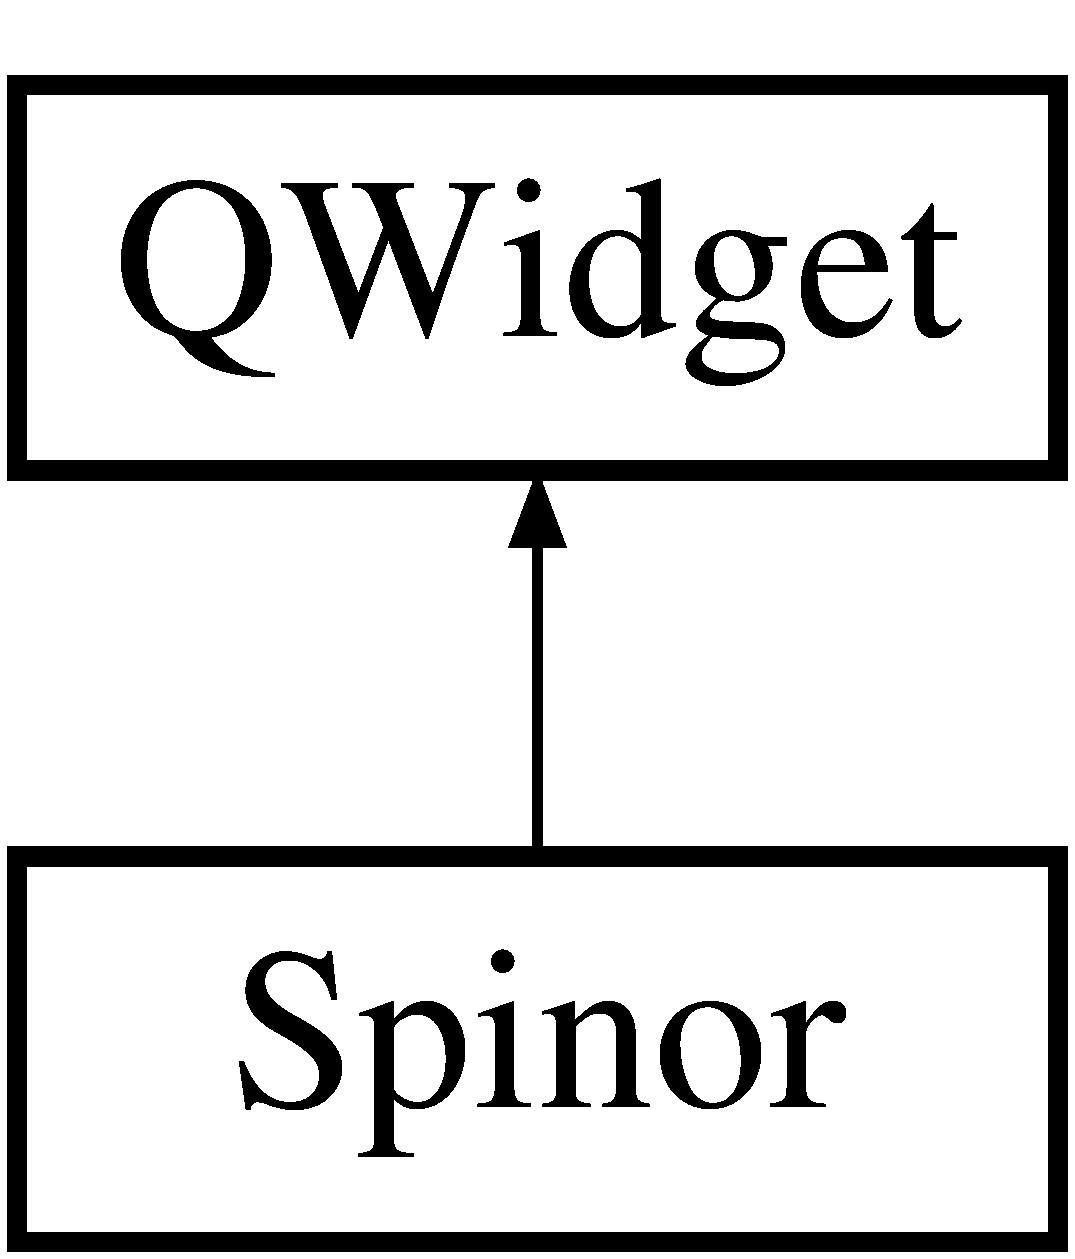
\includegraphics[height=2.000000cm]{class_spinor}
\end{center}
\end{figure}
\subsection*{Public Slots}
\begin{DoxyCompactItemize}
\item 
void {\bfseries reset} ()\hypertarget{class_spinor_a372c8663dc0dc9e049a21fc6c6f37210}{}\label{class_spinor_a372c8663dc0dc9e049a21fc6c6f37210}

\end{DoxyCompactItemize}
\subsection*{Public Member Functions}
\begin{DoxyCompactItemize}
\item 
{\bfseries Spinor} (Q\+Widget $\ast$parent=0)\hypertarget{class_spinor_a9cf70803a5de9d0378393a8aebbd786e}{}\label{class_spinor_a9cf70803a5de9d0378393a8aebbd786e}

\item 
void {\bfseries paint\+Event} (Q\+Paint\+Event $\ast$event)\hypertarget{class_spinor_a7e78356e4fd2551c50f6f91b6864473a}{}\label{class_spinor_a7e78356e4fd2551c50f6f91b6864473a}

\item 
void {\bfseries key\+Press\+Event} (Q\+Key\+Event $\ast$e)\hypertarget{class_spinor_af87a826426a3ab81bf0010df8154d756}{}\label{class_spinor_af87a826426a3ab81bf0010df8154d756}

\item 
void {\bfseries set\+\_\+angle} (double value)\hypertarget{class_spinor_a9c5ecfa1d2c4ebda243bcf8e37370f78}{}\label{class_spinor_a9c5ecfa1d2c4ebda243bcf8e37370f78}

\item 
Q\+Push\+Button $\ast$ {\bfseries get\+\_\+win} () const \hypertarget{class_spinor_af8a3f6f57cdbf8034188b897001a10b1}{}\label{class_spinor_af8a3f6f57cdbf8034188b897001a10b1}

\item 
Q\+Push\+Button $\ast$ {\bfseries get\+\_\+lose} () const \hypertarget{class_spinor_ab8e067d4da4f715d97af31e7a8ff5323}{}\label{class_spinor_ab8e067d4da4f715d97af31e7a8ff5323}

\item 
void {\bfseries slab1sety} (double value)\hypertarget{class_spinor_ae886a43cfaee130423b0245831e1961f}{}\label{class_spinor_ae886a43cfaee130423b0245831e1961f}

\item 
void {\bfseries slab2sety} (double value)\hypertarget{class_spinor_a55fddbe02abe0cfbefa31a5d68db4a59}{}\label{class_spinor_a55fddbe02abe0cfbefa31a5d68db4a59}

\item 
void {\bfseries slab1setwidth} (double value)\hypertarget{class_spinor_ab273d29515d167fd984d7374023ed9ea}{}\label{class_spinor_ab273d29515d167fd984d7374023ed9ea}

\item 
void {\bfseries slab2setwidth} (double value)\hypertarget{class_spinor_a57705083ced0350d418109cd7e49b26c}{}\label{class_spinor_a57705083ced0350d418109cd7e49b26c}

\item 
double {\bfseries slab1getwidth} () const \hypertarget{class_spinor_abc0271f517dfc036721c25691ffa4a52}{}\label{class_spinor_abc0271f517dfc036721c25691ffa4a52}

\item 
double {\bfseries slab2getwidth} () const \hypertarget{class_spinor_ad3cd3fcb8b01cb56a8cdfff0300db92a}{}\label{class_spinor_ad3cd3fcb8b01cb56a8cdfff0300db92a}

\item 
double {\bfseries slab1gety} () const \hypertarget{class_spinor_af2c89fd0474d6b70afa2717bae75cbcc}{}\label{class_spinor_af2c89fd0474d6b70afa2717bae75cbcc}

\item 
double {\bfseries slab2gety} () const \hypertarget{class_spinor_adc2abf189b906e5cc09bf2401443c82c}{}\label{class_spinor_adc2abf189b906e5cc09bf2401443c82c}

\item 
void {\bfseries set\+\_\+speed} (double value)\hypertarget{class_spinor_ae457be187533d33c962069b6a07910d1}{}\label{class_spinor_ae457be187533d33c962069b6a07910d1}

\item 
void {\bfseries go} ()\hypertarget{class_spinor_a8f3b58ed9e6ac776c2220285929c3d56}{}\label{class_spinor_a8f3b58ed9e6ac776c2220285929c3d56}

\item 
bool {\bfseries slab1\+\_\+touch} () const \hypertarget{class_spinor_a078fa4cc0da25c2462011aad86a46ade}{}\label{class_spinor_a078fa4cc0da25c2462011aad86a46ade}

\item 
bool {\bfseries slab2\+\_\+touch} () const \hypertarget{class_spinor_ae19d75e01ffdb55760061a8802a4f897}{}\label{class_spinor_ae19d75e01ffdb55760061a8802a4f897}

\item 
void {\bfseries wewon} ()\hypertarget{class_spinor_a94b7ddae393b5392a5536aa0a41792bd}{}\label{class_spinor_a94b7ddae393b5392a5536aa0a41792bd}

\item 
void {\bfseries welost} ()\hypertarget{class_spinor_a81121583e4e11be82469658a921852a1}{}\label{class_spinor_a81121583e4e11be82469658a921852a1}

\item 
Q\+Push\+Button $\ast$ {\bfseries getwin} () const \hypertarget{class_spinor_a83ba00ed91422e5a5bf4a4c8836be441}{}\label{class_spinor_a83ba00ed91422e5a5bf4a4c8836be441}

\item 
Q\+Push\+Button $\ast$ {\bfseries getlose} () const \hypertarget{class_spinor_a55065887807a2dd0839421cce0358546}{}\label{class_spinor_a55065887807a2dd0839421cce0358546}

\item 
bool {\bfseries lost} () const \hypertarget{class_spinor_a4b524e411ecf137b2991eecb1d927d26}{}\label{class_spinor_a4b524e411ecf137b2991eecb1d927d26}

\item 
bool {\bfseries won} () const \hypertarget{class_spinor_aa3d89dc20f4dc1fdde62ce578cde2756}{}\label{class_spinor_aa3d89dc20f4dc1fdde62ce578cde2756}

\end{DoxyCompactItemize}


The documentation for this class was generated from the following files\+:\begin{DoxyCompactItemize}
\item 
Spinor.\+h\item 
Spinor.\+cpp\end{DoxyCompactItemize}

%--- End generated contents ---

% Index
\backmatter
\newpage
\phantomsection
\clearemptydoublepage
\addcontentsline{toc}{chapter}{Index}
\printindex

\end{document}
